\documentclass{article}
\usepackage{graphicx}
\usepackage{lipsum}
\usepackage[breakable]{tcolorbox}
\usepackage{tcolorbox}
\usepackage{xcolor}
\usepackage{hyperref}
\usepackage{indentfirst}
\usepackage{amsmath}
\usepackage{cite}
\usepackage{caption}
\usepackage{subcaption}

\newtcolorbox{stretchbox}[1][]{
  height fill,
  sharp corners,
  colback=white!10!white,
  colframe=black!50!black,
  #1}

\begin{document}
	
%------------------------------------TITLE PAGE------------------------------------------------------------------------------------------------
\begin{titlepage}
{
	\begin{center}
		
\includegraphics[width=.2\linewidth]{walchand.jpg}\\[.5cm]
		\textbf{\Large Walchand College of Engineering, Sangli }\\
		\textbf {(An Autonomous Institute)}\\[.5cm]
		 \textbf {\LARGE Department of Computer Science and Engineering}\\[1.5cm]
		{ \large \textbf{ A  Mini- Project Report on} }\\[.5cm]
		\textbf{\Large VirtualCampus: Prototyping 3D Mobile Augmented Reality Systems for Exploring the College campus 	using Android app}\\[1cm]
		\large  \textbf{under the guidance of}\\[.3cm]
		\Large \textbf{Mrs. T. T. Kulkarni  }\\[1cm]
		\large \textbf {Submitted by}\\[.5cm]
%	\end{center}
{\setlength{\tabcolsep}{30pt}
\renewcommand{\arraystretch}{1.5}
		\begin{tabular}{ll}
			\large\textbf{Vaibhav Ananda Kumbhar } & \large\textbf{2012BCS057} 
				%& \large\textbf{vkumbhar94@gmail.com}  
				\\
			\large \textbf{Akshay Shirish Habbu }&\large\textbf{2012BCS095}
				% & \large\textbf{akshayhabbu4@gmail.com}
				\\
			\large\textbf{Machchindra Sanjay Pol} & \large\textbf{2012BCS091}
				% &  \large\textbf{machchindrapol@gmail.com}
				\\
		\end{tabular}\\[1.5cm]
}

%	\begin{center}
		\vfill
		\large \textbf{2014-2015 }\\[.4cm]
	\end{center}
}
\end{titlepage}


%-------------------------------------------CERTIFICATE-----------------------------------------------------------------------------
\newpage
%\begin{titlepage}
%\begin{stretchbox}
{	
\linespread{1.6}

	\begin{center}
		
\includegraphics[width=.2\linewidth]{walchand.jpg}\\[.5cm]
		\textbf{\Large Walchand College of Engineering, Sangli }\\
		\textbf {(An Autonomous Institute)}\\[.5cm]
		 \textbf {\LARGE Department of Computer Science and Engineering}\\[1cm]
		\huge \textbf{\textcolor{blue}{\underline{CERTIFICATE}}}\\[1cm]
	\end{center}
		\par \large This is to certify that the Third Year B.Tech. project entitled VirtualCampus: Prototyping 3D Mobile Augmented Reality Systems for Exploring the College campus using Android app is a bonafied work carried out by the student team- 
	\textbf{ Mr. Vaibhav Anand Kumbhar}  , \textbf{ Mr. Machchindra Sanjay Pol } and \textbf{  Mr .Akshay Shirish Habbu }  - 
in partial fulfillment of the completion of 5th semester B. Tech. course during the year 2012 – 2013. The project report has been approved as it satisfies the academic requirement with respect to the project work.\\[2cm]
\vfill
\begin{minipage}{.5\linewidth}
	\begin{flushleft}
		\textbf{Guide}\\
		\textbf{Mrs. T. T. Kulkarni}\\
	\end{flushleft}
\end{minipage}
\begin{minipage}{.5\linewidth}
	\begin{flushright}
	
	\textbf{H.O.D}\\
	\textbf{Dr. B. F. Momin}\\
	\end{flushright}
\end{minipage}

%\end{stretchbox}

%\end{titlepage}
}


%----------------------------------Contents--------------------------




\newpage
{
\tableofcontents
}
\newpage
\listoffigures
%\setcounter{secnumdepth}{-2}% default for "report" is 2



%---------------------------------ABBREViATIONS-------------------------
\newpage
\begin{center}
	\LARGE ABBREVIATIONS
\end{center}

\renewcommand\arraystretch{1.3}
\renewcommand\tabcolsep{1cm}


\begin{tabular}{| l | l |}
	\hline
	Abbreviation & Meaning\\
	\hline
	AR & Augmented Reality\\
	NFT & Natural Feature Tracking\\
	SDK & Software Development Kit\\
	CV & Computer Vision\\
	POI & Point of Interest\\
	ADE & ARchitect Desktop Engine\\
	\hline
\end{tabular}





%-----------------------------------------------ACKNOWLEGEMENT
\newpage
%\section{Acknowledgements}
\begin{center}
{\LARGE \textbf{ ACKNOWLEGEMENT}}\\[1cm]
\end{center}
{\Large
	\par We wish to take this opportunity to express our deep gratitude to all the people who have 
extended their cooperation in various ways during my project work. It is our pleasure to acknowledge 
the help of all those individuals. 
	\par We would like to thank our project guide Mrs. T. T. Kulkarni mam, Computer Science and 
engineering Department for her guidance and help throughout the development of this project work 
by providing us with required information. With her guidance, cooperation and encouragement we 
had learnt many new things during our project tenure. 
	\par We specially thank Dr. B. F. Momin Head, Computer Science and Engineering Department for 
his continuous encouragement and valuable guidance in bringing shape to this dissertation. 
	\par  We specially thank Dr. G.V. Parishwad Director of Walchad College of Engineering Sangli for 
his encouragement and support.  
	\par In completing this project successfully all our faculty members have given an excellent 
cooperation by guiding us in every aspect. We also thank our lab faculty and librarians.
}\\[1cm]
\vfill

\begin{flushright}
\begin{minipage}{.5\linewidth}

\begin{tabular}{rr}
	\large Kumbhar Vaibhav A. &\large [2012BCS057]\\
	\large Pol Machchindra  S. &\large [2012BCS091] \\
	\large Habbu Akshay S. &\large [2012BCS095]\\
\end{tabular}
\end{minipage}
\end{flushright}




%-----------------------------------------------ABSTRACT------------------------------------------------------------
\newpage
%\section{Abstract}
\begin{center}
{\LARGE \textbf{ ABSTRACT}}\\[1cm]
\end{center}
{\large
	\par Our College premises are rapidly developing with so many departments and so many laboratories with multi-disciplinary environment. For any student, teachers and staff members it will be great if all the related information regarding any infrastructure in the college is being shown on their smartphones. So our project is the same Android application which will display every single information related to the scene that being recorded by the users smartphone i.e. Names of every buildings, labs, departments, offices, open spaces, etc. 
	\par We describe a project work that combines together the overlaid 3D graphics of augmented reality with the untethered freedom of mobile computing. The goal is to explore how these two technologies might together make possible portable android application that can support users in their everyday interactions with the world. We introduce an application that presents information about our college campus, using a mobile phone installed with our android application. We provide an illustrated explanation of how our project is used, and describe our rationale behind designing its software infrastructure.
} 



%-----------------------------------------------Introduction-----------------------------------------------------------------
\newpage
\large
\section{Introduction}
\par The field of Augmented Reality (AR) has existed for just over one decade, but the growth and progress in the past few years has been remarkable. 
\subsection{Augmented Reality?}
\par The basic goal of an AR system is to enhance the users perception of and interaction with the real world through supplementing the real world with 3D virtual objects that appear to coexist in the same space as the real world.  Many recent papers broaden the definition of AR beyond this vision, but in the spirit of the original survey we define AR systems to share the following properties: 

\begin{enumerate}
\item  Blends real and virtual, in a real environment 
\item  Real-time interactive 
\item  Registered in 3D 
\end{enumerate}

\par We describe a project work that combines together the overlaid 3D graphics of augmented reality with the untethered freedom of mobile computing. The goal is to explore how these two technologies might together make possible portable android application that can support users in their everyday interactions with the world. We introduce an application that presents information about our college’s campus, using a mobile phone installed with our android application. We provide an illustrated explanation of how our project is used, and describe our rationale behind designing its software infrastructure. \\


\subsection{Problem definition}
\par Think of a situation where we are moving in any new premises of any college and you need to know every single information about that place. So in the conventional method of current scenario we will google the information about the place not so sure we will either can also go to google maps but the problem is the real time scene and infrastructure you are experiencing is way much different than the conventional maps will show you. So this is how you come to a situation where you can use this kind of app which will show you the real time buildings with names and details on your mobile screen.


%------------------------------------Technical Specification-----------------------------------------------------------------

\newpage
\section{TECHICAL SPECIFICATIONS}

\subsection{Introduction to Augmented Reality }

\iffalse
\subsubsection{History of Augmented Reality}
\par \textbf{1966} Invented Head-Mounted Display which was the first step in making AR a possibility.
\par \textbf{1992}
\begin{itemize}
\item Coined the term “Augmented Reality”.
\item Developed Complex Software at Boeing  to help technicians assemble cables into aircraft.
\end{itemize}
\par \textbf{1999}
\begin{itemize}
\item In 1999, Hirokazu Kato of the Nara Institute of Science and Technology released the ARToolKit to the open source community.
\item Although the smartphone was yet to be invented, it was what allowed a simple, handheld device with a camera and an internet connection to bring AR to the masses.
\end{itemize}

\fi

\subsubsection{What is Augmented reality? }
\par Augmented reality is the display of computer graphics and media, overlaid and registered on real-world environments, interactively in real time.{\small{In other words,}}
\par Augmented reality (AR) is the act of enhancing reality with computer-generated content that, in this case, is activated by holding a “marker” in front of a webcam.

\subsubsection{Uses of Augmented Reality}
\begin{itemize}
\item Archaeology
\item Architecture
\item Art
\item Commerce
\item Education
\item Gaming
\item Military
\item Navigation
\item Translation
\end{itemize}


\subsection{ Features and Concepts of Wikitude: }

\subsubsection{Image Recognition }
\par Image recognition helps to recognize images in the viewfinder and overlay it with images. Furthermore it shows how to recognize multiple different images and how to react on user clicks on the overlaid elements. 
\par The image recognition engine developed by Wikitude is based on the Natural Feature Tracking (NFT) principle. As the name implies, this particular field of computer vision (CV) uses natural features to track images. The alternate approach is the use of marker tracking, which uses artificial images, barcodes for example, to track a scene using artificial shapes. 

\par To implement image recognition engine several steps need to execute: 
\begin{enumerate}
\item \textbf{Preprocessing:} The target image that should be tracked is analyzed. Significant areas in the image, so called Feature Points, are extracted and stored. How the Feature Points are detected and stored is the essential essence of the algorithm used. The preprocessing step is executed only once per tracked image, and can run offline and asynchronously.

\item \textbf{Feature Point Detection:}  On the device, similar to the preprocessing step, the current camera image is analyzed for keypoints. 

\item \textbf{Tracking: } These recognized keypoints are then compared with the keypoints generated from the target images in step 1. If a pre-defined similarity is determined, the image is considered a positive match and then tracked. Several algorithms exist to determine a threshold of similarity, which one to chose is up to the implementation. 
\end{enumerate}
\par These are few terms which defines the Wikitude concepts about AR. 

\begin{itemize}
\item \textbf{Target:}  A target image and its associated extracted data that is used by the tracker to recognize an image. 
\item \textbf{Target collection:}  An archive storing a collection of targets that can be recognized by the tracker. A target collection can hold up to 1000 targets.
\item \textbf{Tracker: }  The tracker analyzes the live camera image and detects the targets stored in its associated target collection. Multiple trackers can be created, however only one tracker can be active for recognition at any given time. 
\end{itemize}


\iffalse
\subsubsection{3D Models}
\par Wikitude also helps to augment a target image with 3D content. It starts by displaying a 3D model on a target and advances by adding displayed animations and interactivity.
\par 3D content within Wikitude can only be loaded from Wikitude 3D Format files (.wt3). This is a compressed binary format for describing 3D content which is optimized for fast loading and handling of 3D content on a mobile device. You still can use 3D models from your favourite 3D modelling tools (Autodesk® Maya® or Blender) but you'll need to convert them into the wt3 file format. The Wikitude 3D Encoder desktop application (Windows and Mac) encodes your 3D source file. The Encoder can handle Autodesk® FBX® files (.fbx) and the open standard Collada (.dae) file formats for encoding to .wt3. 
\par 3D content is rendered on top of 2D objects. This limitation exists because of some SDK internal restrictions. 
\par Four flavours of 3D model AR: 
\begin{enumerate}
\item  3D Model on Target Image
\item Appearing Animation 
\item Interactivity
\item Snap to Screen 
\end{enumerate}
\fi

\subsubsection{POINT OF INTEREST (POI) }
\par The Point Of Interest (POI) will show how you can create a marker that is placed at a specific geolocation. The example is split into four different parts that depend on each other. You will have a complete and reusable marker at the end of the series which has a title, description, a selected and an idle state which animates smoothly from one to another. 
\par Four flavours of POI:
\begin{enumerate}
\item POI at Location 
\item POI with Label 
\item Multiple POIs 
\item Selecting POIs
\end{enumerate}

\subsubsection{RETRIEVING POI DATA }
\par There are several ways to request and work with POI detail information in an ARchitect World. Depending on your application and use case, one might fit better than the other. 
\par Retrieving data consists of three parts 
\begin{enumerate}
\item From Application Model
\item From a Local Resource 
\item From a Webservice
\end{enumerate}
\par Displaying numerous POIs in the camera is a challenge. How many POIs should be offered? How to deal with POIs in same direction? What is the maximum range to show POIs and how to display a long description? The following example cover frequently asked questions related to the POI browser use case and consists of five parts plus a bonus section :
\begin{enumerate}
\item  Presenting Detail
\item POI and AR Radar 
\item  Limiting Visible POIs 
\item Reloading POI Data
\item  Native Detail Screen 
\item Capture Screen Bonus 
\end{enumerate}


\iffalse
\subsubsection{VIDEO DRAWABLES }
\par Besides images, text and HTML content you are able to display videos in augmented reality using the Wikitude SDK. With the help of AR.VideoDrawables you can add a video on top of any target image (AR.Trackable2DObject) or have it displayed at any geo location (AR.GeoObject). Like any other drawable you can position, scale, rotate and change the opacity of the video drawable.\\[.4cm]
\fi

\iffalse
\textbf{SUPPORTED VIDEO CODECS AND HOSTING SERVICES }
\par To support all platforms make sure to use a H.264 encoded video with a maximum resolution of 720p (1280x720 pixel). 
\par H.264 defines different profiles. Make sure that you are using either one of the following :
\begin{itemize}
\item Baseline 
\item Extended 
\item Main 
\end{itemize}

\par If the profile differs Android devices will most certainly misbehave (fail to play or crash entirely) when playing back those videos. 
\par If you like to add a YouTube video, which is then played full-screen in the native player, rather use an AR.ImageDrawable showing a poster or play-button and add the URL to the YouTube video to the onClick trigger. Similar to what we do in the image recognition sample.\\[.4cm]
\par \textbf{VIDEO SAMPLE }\\
\fi


\par This is the way to augment a target image. Furthermore it shows how to react on playback states and concludes with how to use transparent videos. 
\par So it consists of four parts :
\begin{enumerate}
\item Select a Video and add it to a Target Image 
\item Control Video Playback 
\item  Snapping Video 
\item Transparent Video 
\end{enumerate}

\subsubsection{IMAGE RECOGNITION AND GEO }
\par The Wikitude SDK allows you to combine location based augmented reality scenes with vision baed scenes to create a seamless experience for users. This tutorial will show you how to accomplish this and will provide you with additional advices. 

\subsection{ Project Architecture }
\subsubsection{DEVELOPMENT WORKFLOW }
\par The following section describes a default development workflow for writing AR content using the ARchitect JavaScript API. It demonstrates the code test and debug cycle and provides useful tips for each step. \\
\textbf{CODE, TEST, DEBUG :}

\begin{enumerate}
\item Write your HTML, JavaScript and CSS using the text editor of your choice 
\item Test in your desktop browser 
\item Debug in your desktop browser using e.g. WebInspector
\item Test on a physical device
\item Debug on a physical device
\item Rinse and repeat 
\end{enumerate}
\par You can use any editor for writing the ARchitect World. We particularly like Sublime, which has a great selection of plugins for web developers.
\par The next step is to test it out in a desktop browser. To have the ARchitect JavaScript API available in the desktop browser you'll need to include the ARchitect Desktop Engine (ADE). See the chapter ARchitect Desktop Engine for instructions on how to use it. While this is limited in visualizing the experience, it greatly helps in finding errors in the JavaScript code and reduces the time it takes to see effects of changes you have made to the HTML and CSS parts. Desktop browsers come with great debugging tools that allow you to easily debug your JavaScript code and that you should make full use of when debugging ARchitect Worlds. 
\par Once you have verified the JavaScript is working properly you should test it on the device of your choice. Either start your application that loads the ARchitect World or run it inside the Wikitude World Browser app. 
\par AR experiences can be tested on Android using the Wikitude World Browser for Android. Download the Wikitude app from Google Play. Launch the application and press the menu button in the upper left corner of the screen. Then tap the Developer button to open the developer login page. Enter your username and password of your Wikitude developer account and tap the login button to get to your user account. If you don't have a developer account yet register at the Wikitude developer page.
\par In this view, tap on the text box below the Launch via URL label and enter the URL of your ARchitect World. After tapping the Launch button your AR experience will be opened in Wikitude. \\













%-------------------------------------SYSTEM ANALYSIS ---------------------------------------------

\newpage
\section{SYSTEM ANALYSIS }
\subsection{Proposed System: }
\par The proposed system is an android application which detects the places around the entire campus using augmented reality algorithms. The live stream of video data i.e. set of continuous images is fetched to the system, system then identifies the markers in the images and displays the appropriate response back on the live screens. So basically it’s a real time detection of places and it displays back the stored information about that particular place/ markers. 
\par The VirtualCampus app is just a simple single screened application which directly jumps on to your camera view and starts detecting the live frames.   



\subsection{Overview }
\par VirtualCampus is an android application that is been developed using Wikitude SDK. Wikitude is a mobile augmented reality software which is developed by the Austrian company Wikitude GmbH (formerly Mobilizy GmbH) and was first published in October 2008 as freeware. It displays information about the users' surroundings in a mobile camera view, including image recognition and 3d modeling. Wikitude was the first publicly available application that used a location-based approach to augmented reality. 




\subsection{Harware Requirements}
\par To work with project the following hardwares are required:
\begin{itemize}
\item Smart Phone with Android Operating System ,Camera, GPS.
\end{itemize}

\subsection{Software Requirements}
\par List of Softwares needed:
\begin{itemize}
\item Android Studio.
\item ADB Device Support Driver.
\end{itemize}


%----------------------------------SYSTEM DESIGN -----------------------------------------------------
\newpage
\section{SYSTEM DESIGN }
\subsection{Core concepts }
\par As we will show later, many tracking algorithms can be split into functional blocks or even atomic operations which can be reused in other algorithms. The data types used to exchange data between these blocks also have certain similarities. To enable combination of different functional blocks we encapsulate these in abstract classes with a fixed interface. The interface consists of only three functions for initialization, execution and de-initialization. A similar abstract class exists for data, which enables us to store it in a global data-set, where it can be accessed by pointer or name reference. We call these abstract classes Action and Data. The connections between the blocks are defined by the dataflow between them. Each Action has a set of keys which is a reference to a data element, which can be retrieved from the data-set before execution. The indirection over a key element for data access allows the use of a graphical interface or a scripting language to setup the data-flow. Actions and Data also provide a reflective type interface to access selected class variables either by their original type or even more general by string. This provides a generic way to access parameters and data at run-time in graphical interfaces.  

\subsection{Parallelization and Synchronization  }
\par In order to support state of the art multi-core and multi-processor systems, the system offers three different levels of parallelization. All threading and synchronization aspects are based on boost::thread library. The lowest level consists in the classical and straight forward multi-threading implementation achieved by the developer to improve performance of a specific algorithm. At this level it is the developers responsibility to implement correct parallel execution. The mid-level is done automatically and is based on dependency analysis of the data flow. 
\par  As a result we get a dependency graph which is used to select Actions with independent data inputs, able to run in parallel without any conflicts. This method can be seen from the outside as a sequential processing and does not require precautions to protect the data from access by simultaneous running threads, due to the precondition of having independent data. The method does not require any knowledge about the algorithm, but relies on a fine granularity in the building blocks, the more atomic they perform their work the more can be parallelized. This method is the easiest to use for the developer, he can develop the tracking system in a clear hierarchical manner (top down) without caring about execution order. Although this method might not produce an optimal result, it is a convenient way to improve performance. 
\par . As a third method, our system provides a Component which is a configuration of Actions, executed in its own thread. This concept is important for tracking with devices running at different framerates, like inertial sensors (e.g. 100Hz) and cameras (e.g. 25Hz). In such a case the sensor interface and a pose estimation algorithm, like a Kalman filter, would run in one component at sensor frame rate, while the slower camera and vision part runs in another component. In order to synchronize data exchange between these components, the data objects incorporate a locking mechanism. The same mechanism also handles signals to notify other components about changes in the data. Additionally our data objects can be time stamped to identify related data in an asynchronous setup, where multiple sensor inputs must be handled.  

\subsection{Extending the System }
\par New Action and Data classes built in to shared libraries can be added to our framework by simply loading them during runtime. This makes the system extendable without rebuilding it and allows enhancements by adding more problem specific Actions while reusing the existing Actions for common processing steps. The system provides a type-factory where all available (linked) object are registered and can be instantiated by name. This comes in useful when reading configurations from a XML file or when composing new configurations with a graphical interface.   

\subsection{Interfacing}
\par To use the system as a library in once own application, only the instantiation of the run-time instance is necessary. It provides access to all Actions and data in the system. By accessing the Actions, all parameters can be varied during run-time. Results or additional input data can be accessed through the global data-set where all data objects are stored. The run-time system also has a singleton which provides a static pointer to itself, which makes access from different  classes easier. The run-time instance provides some general purpose functions useful in any application like loading and saving of xml configuration files, loading of extensions, and it defines abstract entry points for a graphical interface which allows separation of user interface and library. How this concept can be exploited to build certain types of applications, is outlined in the Application Framework section below. 

\subsection{Tracking Framework}
\par In order to simplify the implementation of tracking algorithms and reuse as much code as possible, we define a tracking framework consisting of several base classes representing the major steps in tracking algorithms. We identified the following steps which are common to the most visual 3D tracking systems:
\subsubsection{Common Processing steps- }

\begin{itemize}
\item \textbf{Image processing-}In this, usually the first step, the incoming video images are modified to fit the requirements of the following processing steps. Examples are image and video capture, image read and write to file, gradient image, image pyramid, binarization, image conversion, undistortion, etc. 
\item \textbf{Feature detection-} at this step higher level information such as interest points of an image are generated. This step is specific to a given tracking procedure. Examples are Harris - corner detector, edge detection, KLT - Kanade Lucas tracker - the feature detection part, SURF 
\item \textbf{Tracking, matching or classification-} The process of correspondence determination is very specific to a tracking procedure and can consists in searching features seen in the past images (tracking), comparison with reference data (matching) or feature sorting (classification). Examples for tracking are KLT point tracking, line tracker, for matching features with references there is MSER and for classification we have randomized trees.  
\item \textbf{Pose estimation- } Computation of a camera pose with a given set of correspondences. Examples are generic pose calculation with Kalman Filter, RANSAC (linear or non linear estimation with inliers/outliers tests),POSIT, linear pose calculation: HEIV and nonlinear pose estimation (Levenberg-Marquardt). 
\end{itemize}

\subsection{Data Flow Diagram}
\begin{figure}[h]
	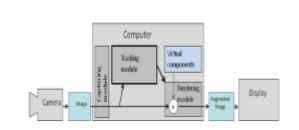
\includegraphics[width=\linewidth]{flowchart.jpg}
	\caption{Flow Chart for a Simple AR System. }
\end{figure}
\begin{figure}[h]
	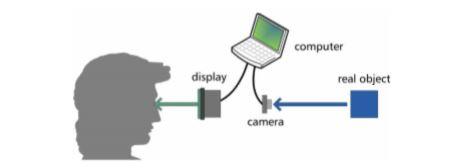
\includegraphics[width=\linewidth]{SimpleAR.jpg}
	\caption{Simple AR System Flow. }
\end{figure}


\subsection{ Output Design }
\par Designing computer output should proceed in an organized, well throughout manner; the right output element is designed so that people will find the system whether or executed. When we design an output we must identify the specific output that is needed to meet the system. The usefulness of the new system is evaluated on the basis of their output. 
\par Once the output requirements are determined, the system designer can decide what to include in the system and how to structure it so that the required output can be produced. For the proposed software, it is necessary that the output reports be compatible in format with the existing reports. The output must be concerned to the overall performance and the system’s working, as it should. It consists of developing specifications and procedures for data preparation, those steps necessary to put the inputs and the desired output, i.e. maximum user friendly. Proper messages and appropriate directions can control errors committed by users.
\par The output design is the key to the success of any system. Output is the key between the user and the sensor. The output must be concerned to the system’s working, as it should. Output design consists of displaying specifications and procedures as data presentation. User is never left with the confusion as to what is happening without appropriate error and acknowledges message being received. Even an unknown person can operate the system without knowing anything about the system. 


%-------------------------------SYSTEM TESTING --------------------------------

\newpage
\section{SYSTEM TESTING }
\subsection{ \textbf{ON-DEVICE DEBUGGING }}
\par Remote debugging is available for devices running Android.
\par{ To enable remote debugging of a WebView add the following line to your CamActivity. }\\[.3cm]
$if(Build.VERSION.SDK\_INT \geq 19) \{\\
WebView.setWebContentsDebuggingEnabled(true);\\
\} $

\par setWebContentsDebuggingEnabled is available for Android 4.4+, you may need to capsule that to avoid runtime errors on devices running Android lower version 4.4. Additionally set TargetSDK to 19 in your Android Manifest.





%------------------------------IMPLEMENTATION-----------------------------------------------------
\newpage
\section{IMPLEMENTATION}
\par Implementation is the stage in the project where the theoretical design is turned into a working system and is giving confidence on the new system for the users that it will work efficiently and effectively. It involves careful planning, investigation of the current system and its constraints on implementation, design of methods to achieve the changeover, an evaluation of change over methods.
\par  Apart from planning major task of preparing the implementation are education and training of users. The implementation process begins with preparing a plan for the implementation of the system. According to this plan, the activities are to be carried out, discussions made regarding the equipment and resources and the additional equipment has to be acquired to implement the new system.
\par  The most critical stage in achieving a successful new system is giving the users confidence that the new system will work and be effective. The system can be implemented only after thorough testing is done and if it is found to be working according to the specification. This method also offers the greatest security since the old system can take over if the errors are found or inability to handle certain type of transactions while using the new system.

\subsection{Recongnition}
\par There is one object of \textbf{Trackable2D}.This object is used for the recognition.
\begin{figure}[h]
	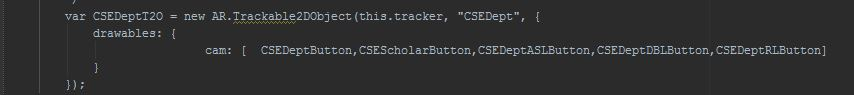
\includegraphics[width=\linewidth]{Trackable2D.jpg}
	\caption{Code Snippet-Trackable2D. }
\end{figure}
{\clearpage
\subsection{Screen Overlay}
\par These objects are used to add virtual world on  camera view.
\begin{figure}[h]
	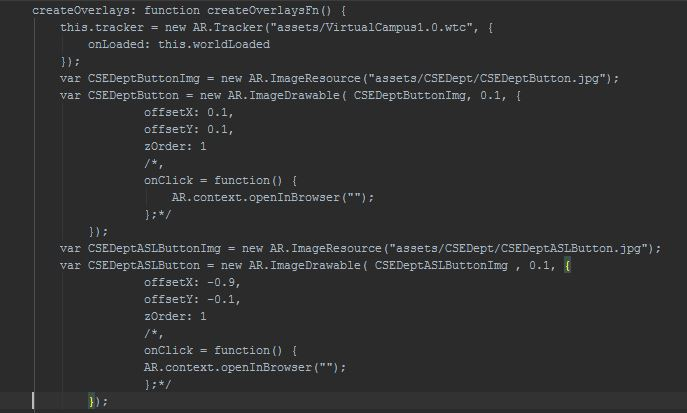
\includegraphics[scale=.5]{ScreenOverlay.jpg}
	\caption{Code Snippet-Overlay Objects. }
\end{figure}
}











%----------------Screenshots and Results-------------------------------------------------------------------------
\pagebreak
\newpage

\section{Screenshots and Results}

\iffalse
\begin{figure}[h]
  \begin{subfigure}[b]{0.4\textwidth}
    
\includegraphics[width=.9\linewidth]{Icon.png}
  	\caption{Application Icon}
    \label{fig:1}
  \end{subfigure}
  %
  \begin{subfigure}[b]{0.4\textwidth}
  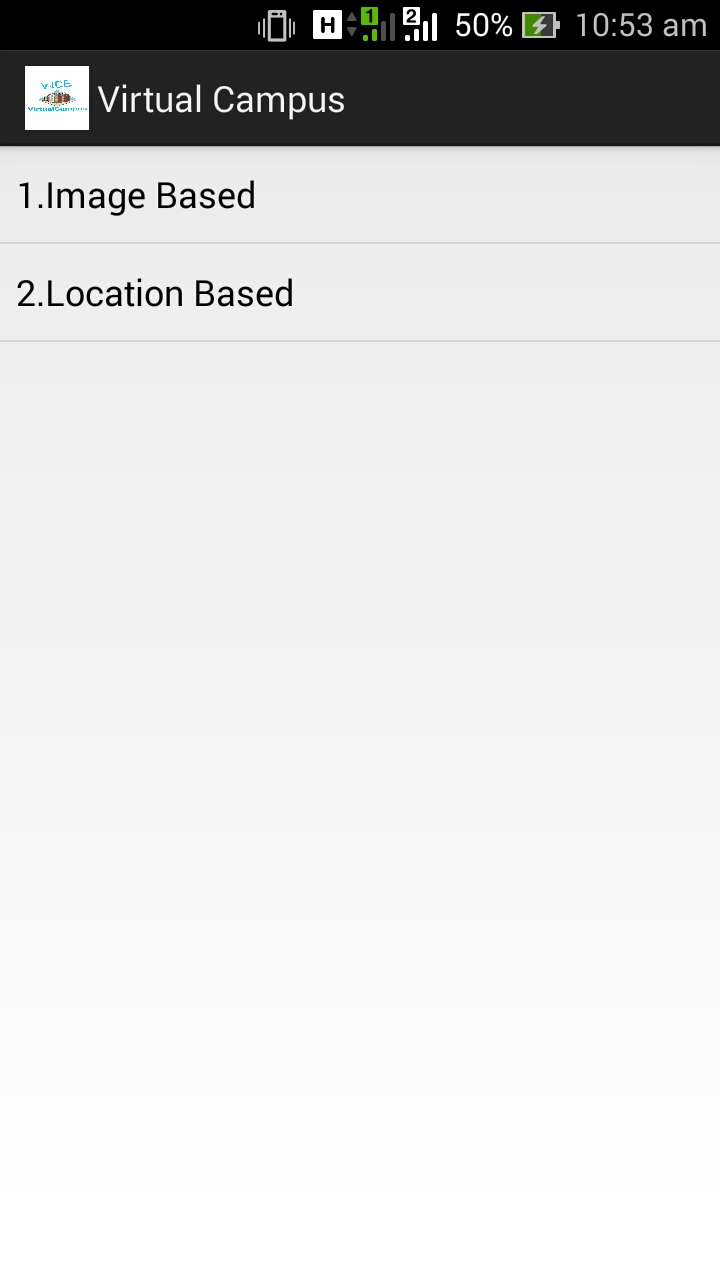
\includegraphics[scale=1,trim=0 50cm 0 0,clip=true]{AppEntryView.jpg}
    \caption{Application Entry View}
    \label{fig:2}
  \end{subfigure}
\end{figure}
\fi


%\iffalse
\begin{figure}[h]
\centering
\begin{minipage}{.5\textwidth}
  \centering
  
\includegraphics[width=.9\linewidth]{Icon.png}
  \captionof{figure}{Application Icon}
  \label{fig:icon}
\end{minipage}%
\begin{minipage}{.5\textwidth}
  \centering
  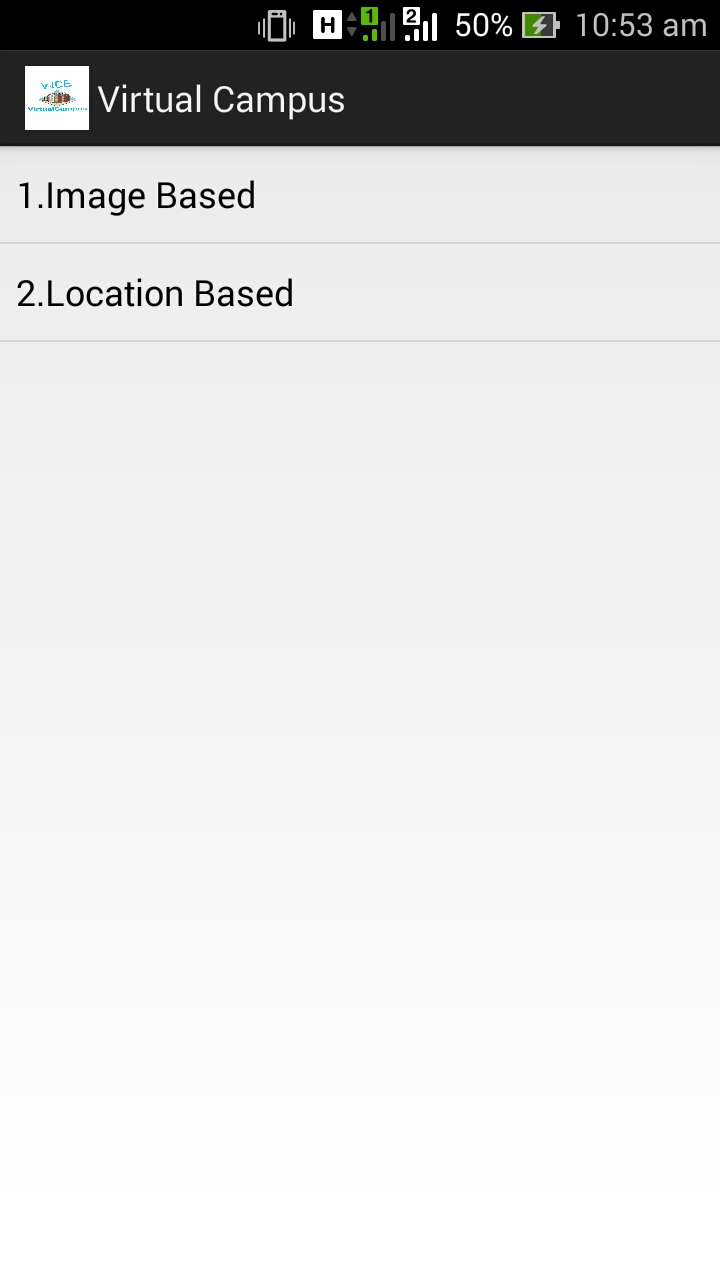
\includegraphics[width=.6\linewidth,height=5cm]{AppEntryView.jpg}
  \captionof{figure}{Application Entry View}
  \label{fig:appentry}
\end{minipage}
\end{figure}
%\fi





\iffalse
%\subsection{Application Icon}
\begin{center}
\begin{figure}[h]
	
\includegraphics[scale=.3]{Icon.png}
	\caption{Application Icon. }
\end{figure}
\end{center}
\vspace{5cm}
%\subsection{Application Entry View}
\begin{center}
\begin{figure}[h]
	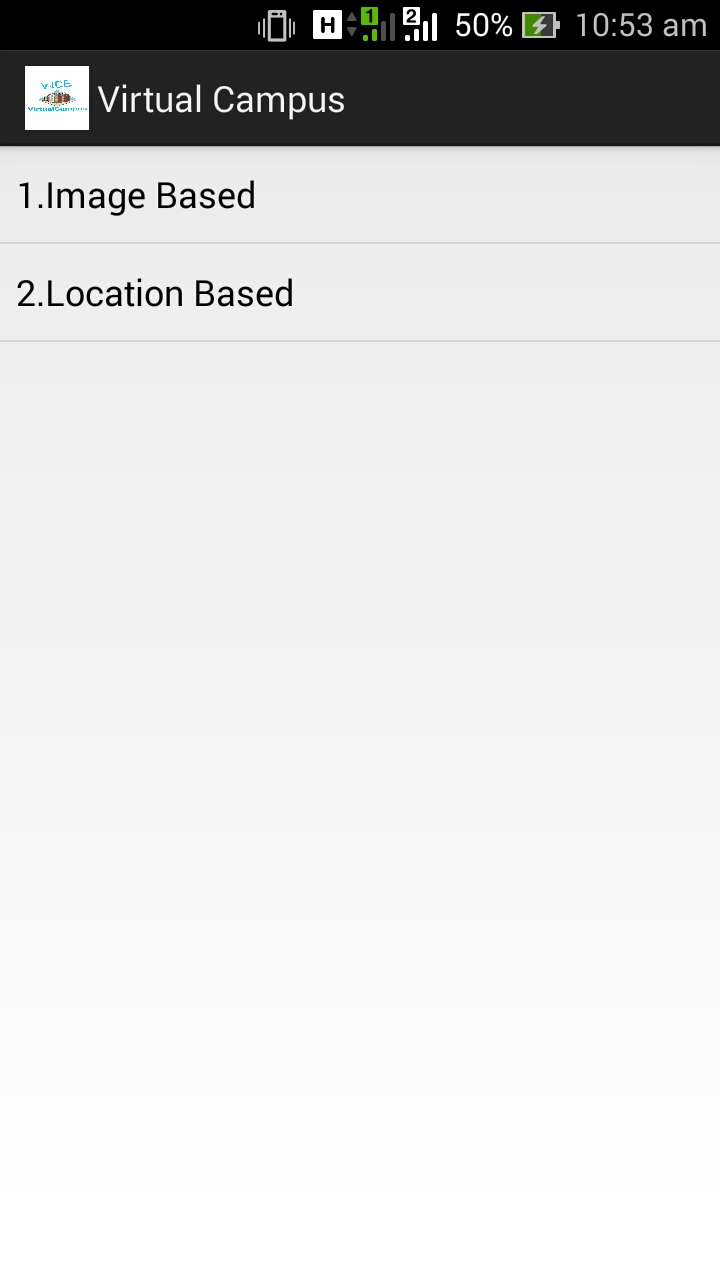
\includegraphics[scale=0.3,trim=0 30cm 0 0,clip=true]{AppEntryView.jpg}
	\caption{Application Entry View. }
\end{figure}
\end{center}
%\subsection{College's Front View Recognition}
\begin{figure}[h]
	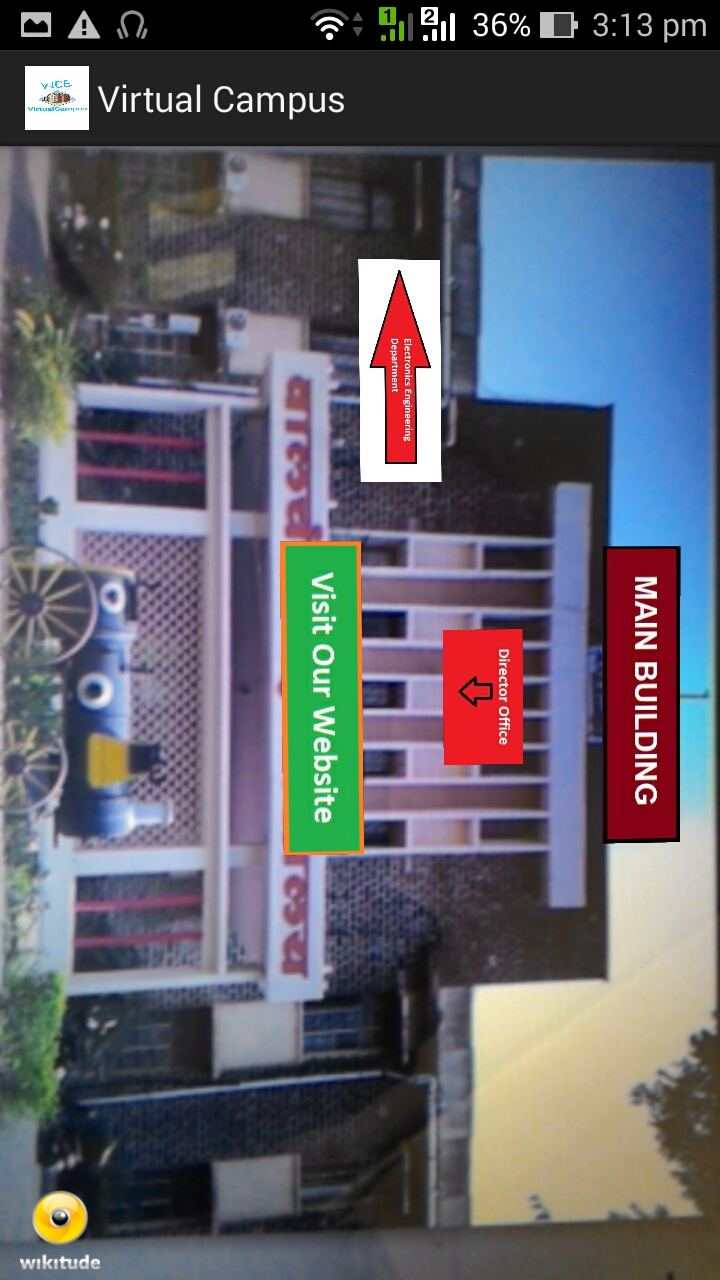
\includegraphics[scale=0.2,angle=90]{MainBuilding.jpg}
	\caption{College's Front View Recognition . }
\end{figure}
\fi

%\subsection{CCF View Recognition}
\begin{figure}[h]
\centering
\begin{minipage}{.5\textwidth}
  \centering
	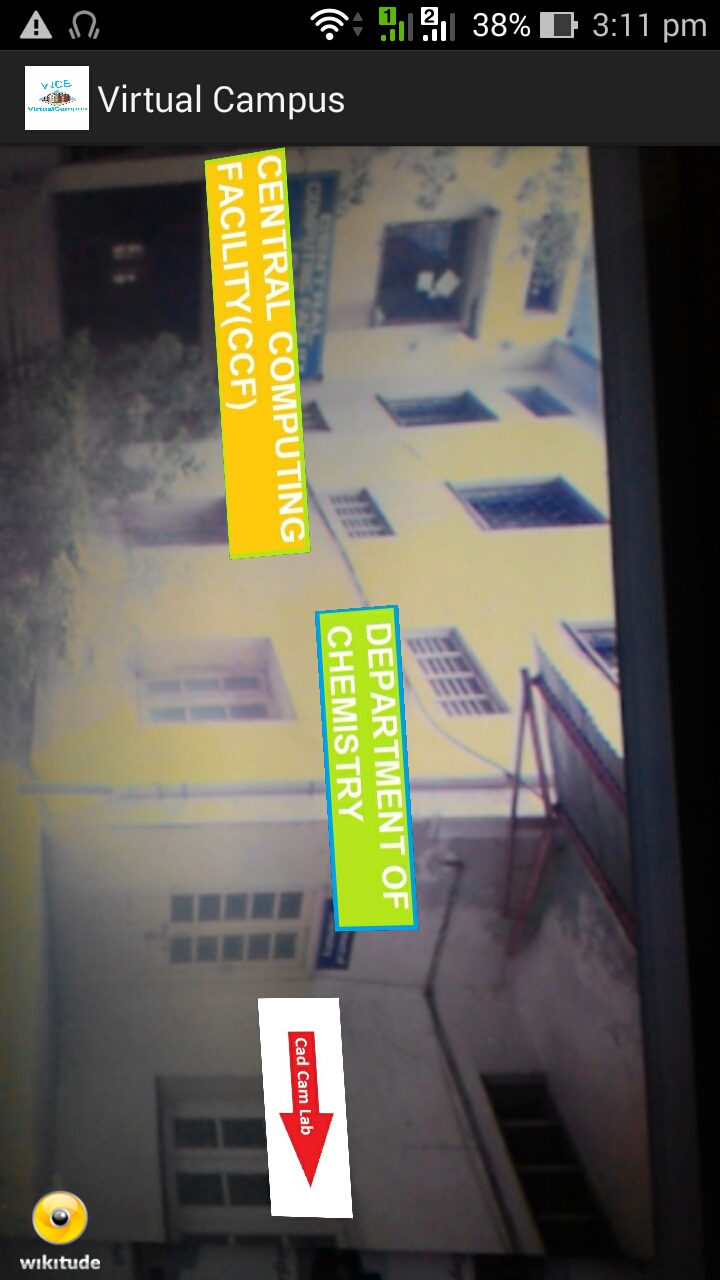
\includegraphics[width=.4\linewidth,angle=90]{CCF.jpg}
 	 \captionof{figure}{CCF View Recognition . }
  \label{fig:ccf}
\end{minipage}%
\begin{minipage}{.5\textwidth}
  \centering
	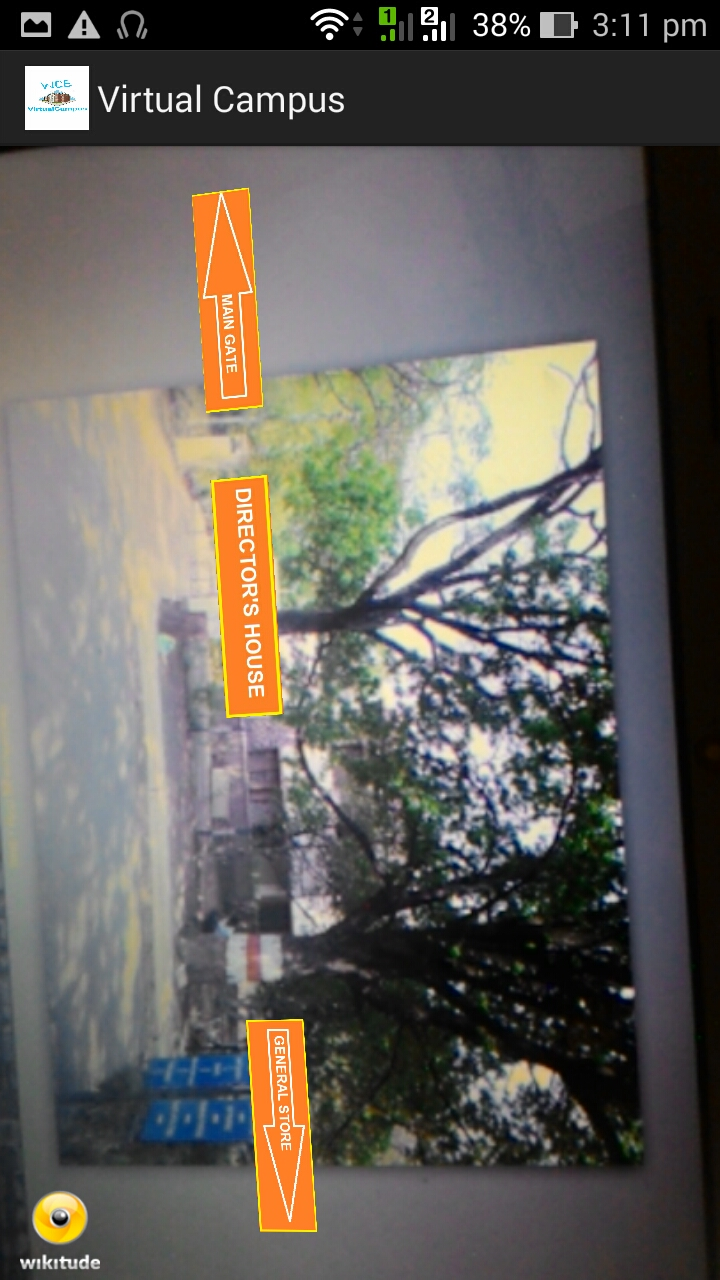
\includegraphics[width=.4\linewidth,angle=90]{DirectorHome.jpg}
	\captionof{figure}{ Director's HouseView Recognition . }
  \label{fig:directorhome}
\end{minipage}
\end{figure}

%\subsection{Director's House View Recognition}


\begin{figure}[h]
\centering
\begin{minipage}{.5\textwidth}
  \centering
	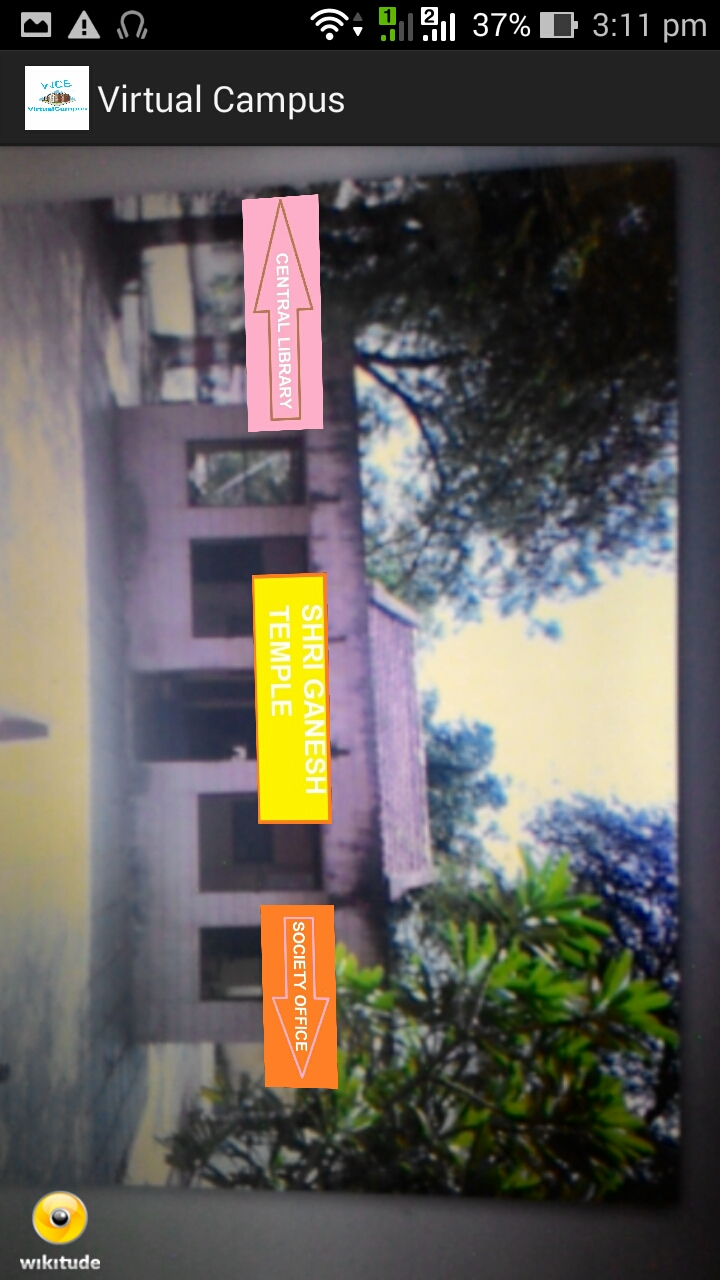
\includegraphics[width=.4\linewidth,angle=90]{GaneshTemple.jpg}
	\captionof{figure}{ Ganesh Temple View Recognition . }
  \label{fig:ccf}
\end{minipage}%
\begin{minipage}{.5\textwidth}
  \centering
	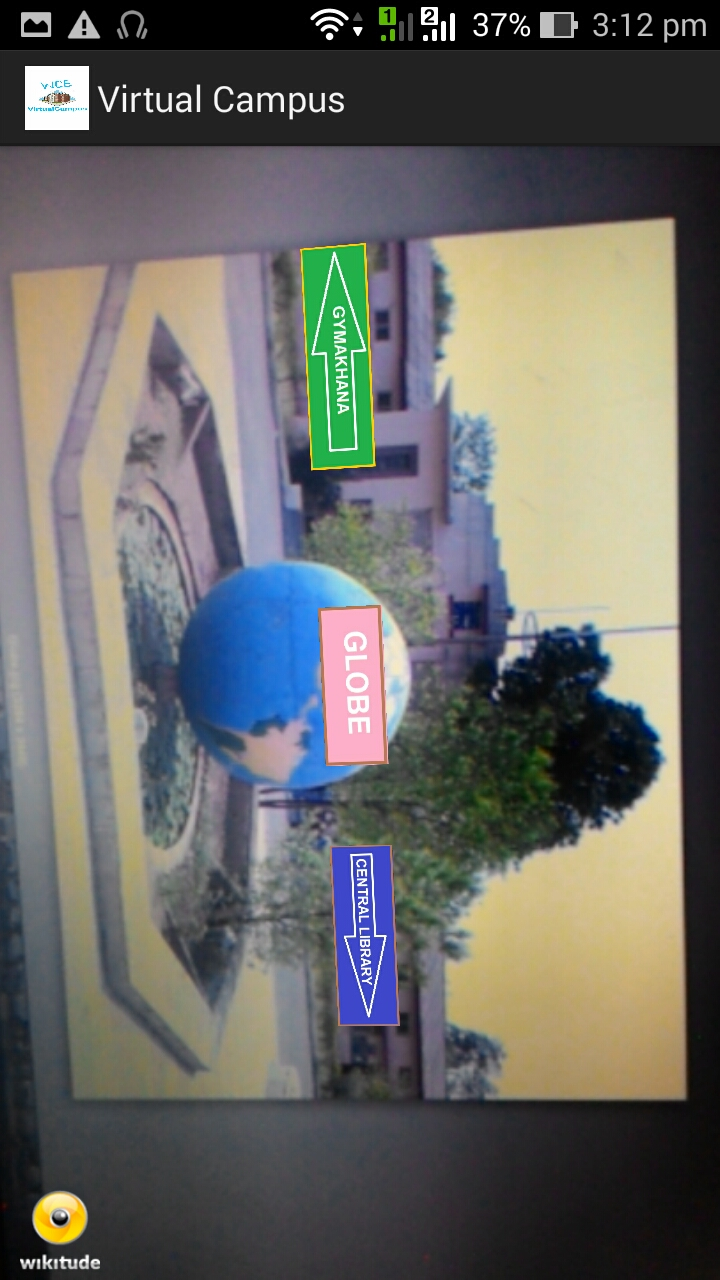
\includegraphics[width=.4\linewidth,angle=90]{Globe.jpg}
	\captionof{figure}{ Globe Recognition . }
  \label{fig:globe}
\end{minipage}
\end{figure}

\begin{figure}[h]
\centering
\begin{minipage}{.5\textwidth}
  \centering
	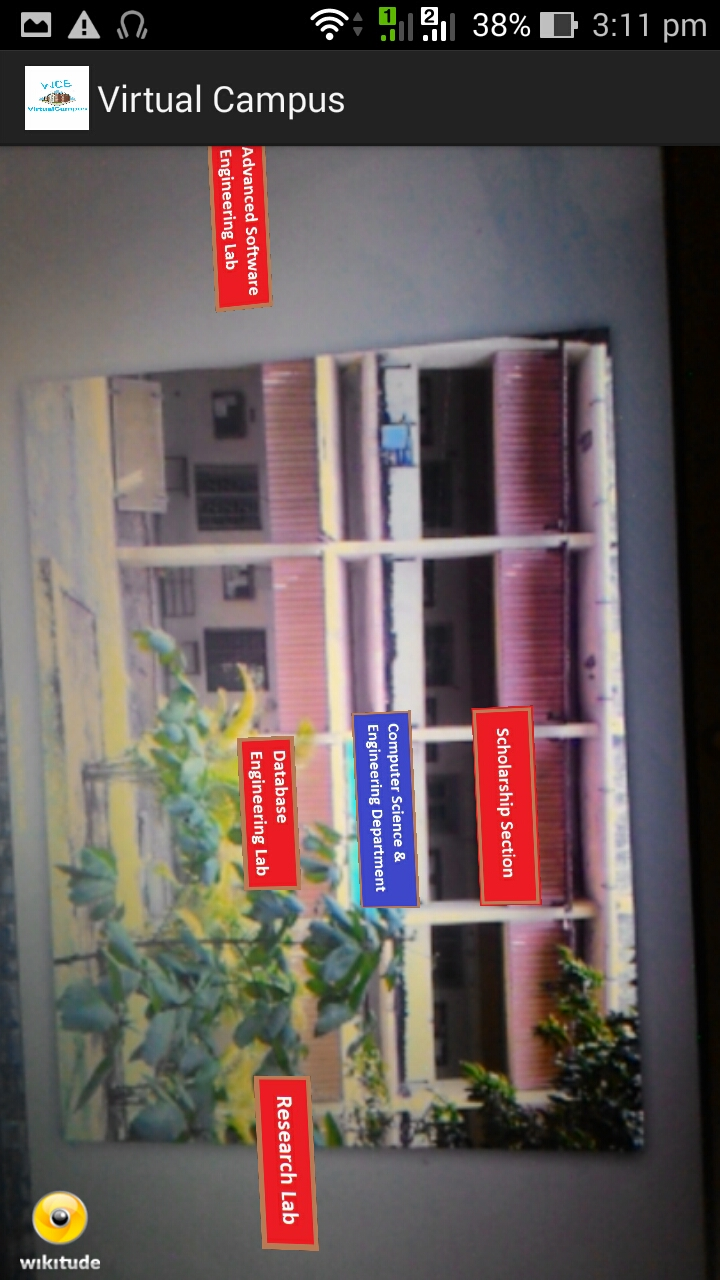
\includegraphics[width=.4\linewidth,angle=90]{CSEDept.jpg}
	\captionof{figure}{ CSE Department View Recognition . }
  \label{fig:csedept}
\end{minipage}%
\begin{minipage}{.5\textwidth}
  \centering
	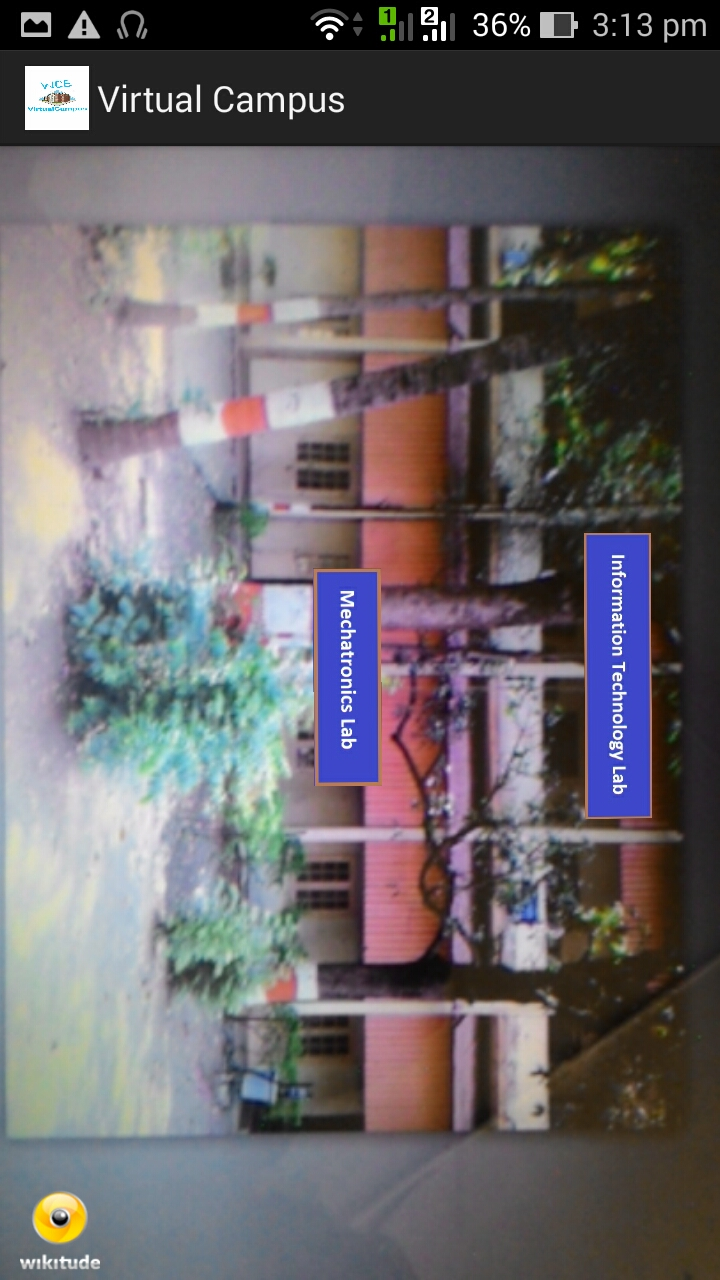
\includegraphics[width=.4\linewidth,angle=90]{ITDept.jpg}
	\captionof{figure}{ IT Department view Recognition . }
  \label{fig:itdept}
\end{minipage}
\end{figure}

\begin{figure}[h]
\centering
\begin{minipage}{.5\textwidth}
  \centering
	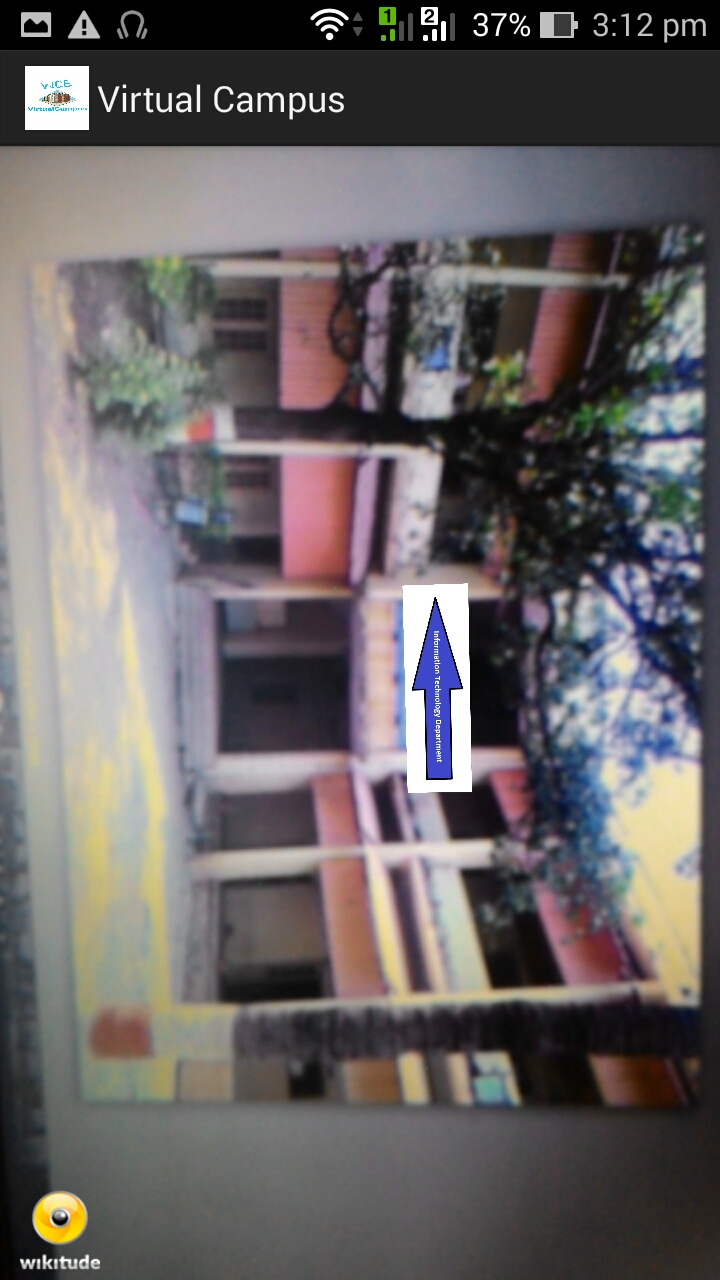
\includegraphics[width=.4\linewidth,angle=90]{IT.jpg}
	\captionof{figure}{ IT Department View Recognition . }
  \label{fig:csedept}
\end{minipage}%
\begin{minipage}{.5\textwidth}
  \centering
	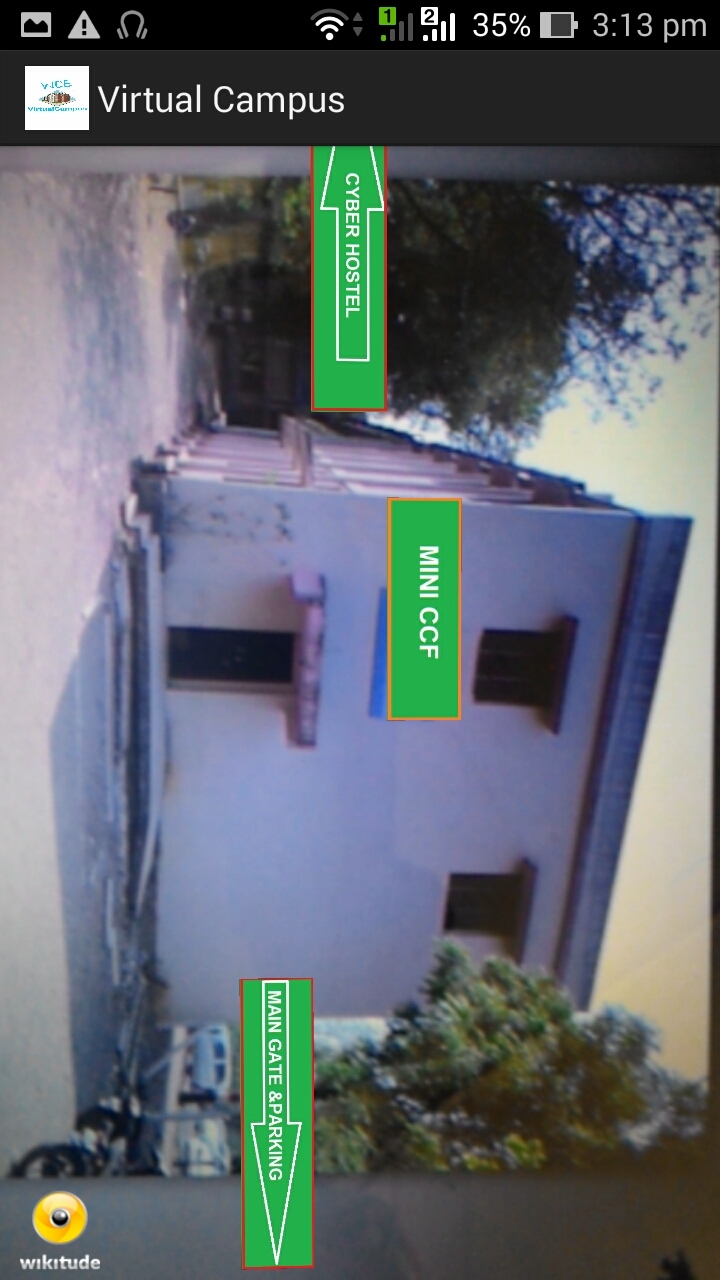
\includegraphics[width=.4\linewidth,angle=90]{MiniCF.jpg}
	\captionof{figure}{ Mini CF view Recognition . }
  \label{fig:itdept}
\end{minipage}
\end{figure}


\clearpage

%\subsection{Ganesh Temple View Recognition}


%------------------------------------Conclusion & Future Work-----------------------------------------------------------

\newpage
\section{Conclusion and Future Work}
\subsection{Conclusion}
\par To conclude the description about the project: The project, developed by Augmented reality SDK- WikiTude using Android for development platform is based on the idea that fascinates our entire team, To make use of the latest technological advancements in day to day life. The idea of embedding the real life scenarios to the virtual world is always the motive behind our project work. This application helps navigating and sharing information about the college campus and the places around it. 
\par The application is a navigation aid to people walking outdoors.  These individuals could be students advancing upon their objective, faculties trying to gain information of the campus, or guests seeking directions to their intended destination.  Today, these individuals must pull out a physical map and associate what they see in the real environment around them with the markings on the 2–D map.  If landmarks are not easily identifiable, this association can be difficult to perform.  An AR system makes navigation easier by performing the association step automatically.  If the user's position and orientation are known, and the AR system has access to a digital map of the area, then the AR system can draw the map in 3-D directly upon the user's view.  The user looks at a nearby buildings and sees graphics directly overlaid on the real environment explaining the building’s name, what are the highlights of it, how far away it is, and List of faculties and students studying etc. 

\subsection{Future Work}
\par Now the space ovehead is on mobile's memory. So in future, We can extend this project with cloud recognition facility. Real time 3D recognition also possible.






\newpage
%\label{Bibliography}
%\bibliographystyle{plain} % Use the "unsrtnat" BibTeX style for formatting the Bibliography
%\bibliography{mybib.bib} 
{\centering \Large \textbf{REFERENCES}}\\[.5cm]
\begin{enumerate}
\item Visual Tracking for Augmented Reality -Georg Klein.
\item Pro Android Augmented Reality  -Raghav Sood.
\item Wikitude.com -Offcial Documentation and User Forum.
\end{enumerate}








\end{document}